%%%%%%%%%%%%%%
%% Run LaTeX on this file several times to get Table of Contents,
%% cross-references, and citations.

%% If you have font problems, you may edit the w-bookps.sty file
%% to customize the font names to match those on your system.

%% w-bksamp.tex. Current Version: Feb 16, 2012
%%%%%%%%%%%%%%%%%%%%%%%%%%%%%%%%%%%%%%%%%%%%%%%%%%%%%%%%%%%%%%%%
%
%  Sample file for
%  Wiley Book Style, Design No.: SD 001B, 7x10
%  Wiley Book Style, Design No.: SD 004B, 6x9
%
%
%  Prepared by Amy Hendrickson, TeXnology Inc.
%  http://www.texnology.com
%%%%%%%%%%%%%%%%%%%%%%%%%%%%%%%%%%%%%%%%%%%%%%%%%%%%%%%%%%%%%%%%

%%%%%%%%%%%%%
% 7x10
%\documentclass{wileySev}

% 6x9
\documentclass{wileySix}

\usepackage{graphicx}
\usepackage{listings}

\usepackage{color}

\definecolor{codegreen}{rgb}{0,0.6,0}
\definecolor{codegray}{rgb}{0.5,0.5,0.5}
\definecolor{codepurple}{rgb}{0.58,0,0.82}
\definecolor{backcolour}{rgb}{0.95,0.95,0.92}

\lstdefinestyle{mystyle}{
    backgroundcolor=\color{backcolour},
    commentstyle=\color{codegreen},
    keywordstyle=\color{magenta},
    numberstyle=\tiny\color{codegray},
    stringstyle=\color{codepurple},
    basicstyle=\footnotesize,
    breakatwhitespace=false,
    breaklines=true,
    captionpos=b,
    keepspaces=true,
    numbers=left,
    numbersep=5pt,
    showspaces=false,
    showstringspaces=false,
    showtabs=false,
    tabsize=2,
    language=sh
}

\lstset{style=mystyle}

%%%%%%%
%% for times math: However, this package disables bold math (!)
%% \mathbf{x} will still work, but you will not have bold math
%% in section heads or chapter titles. If you don't use math
%% in those environments, mathptmx might be a good choice.

% \usepackage{mathptmx}

% For PostScript text
\usepackage{w-bookps}

%%%%%%%%%%%%%%%%%%%%%%%%%%%%%%%%%%%%%%%%%%%%%%%%%%%%%%%%%%%%%%%%
%% Other packages you might want to use:

% for chapter bibliography made with BibTeX
% \usepackage{chapterbib}

% for multiple indices
% \usepackage{multind}

% for answers to problems
% \usepackage{answers}

%%%%%%%%%%%%%%%%%%%%%%%%%%%%%%
%% Change options here if you want:
%%
%% How many levels of section head would you like numbered?
%% 0= no section numbers, 1= section, 2= subsection, 3= subsubsection
%%==>>
\setcounter{secnumdepth}{3}

%% How many levels of section head would you like to appear in the
%% Table of Contents?
%% 0= chapter titles, 1= section titles, 2= subsection titles,
%% 3= subsubsection titles.
%%==>>
\setcounter{tocdepth}{2}

%% Cropmarks? good for final page makeup
%% \docropmarks

%%%%%%%%%%%%%%%%%%%%%%%%%%%%%%
%
% DRAFT
%
% Uncomment to get double spacing between lines, current date and time
% printed at bottom of page.
% \draft
% (If you want to keep tables from becoming double spaced also uncomment
% this):
% \renewcommand{\arraystretch}{0.6}
%%%%%%%%%%%%%%%%%%%%%%%%%%%%%%

%%%%%%% Demo of section head containing sample macro:
%% To get a macro to expand correctly in a section head, with upper and
%% lower case math, put the definition and set the box
%% before \begin{document}, so that when it appears in the
%% table of contents it will also work:

\newcommand{\VT}[1]{\ensuremath{{V_{T#1}}}}

%% use a box to expand the macro before we put it into the section head:

\newbox\sectsavebox
\setbox\sectsavebox=\hbox{\boldmath\VT{xyz}}

%%%%%%%%%%%%%%%%% End Demo


\begin{document}


\booktitle{Cerdas Menguasai Python}
\subtitle{Dalam 24 Jam}

\authors{Rolly M. Awangga\\
\affil{Informatics Research Center}
%Floyd J. Fowler, Jr.\\
%\affil{University of New Mexico}
}

\offprintinfo{Cerdas Menguasai Python, First Edition}{Rolly M. Awangga}

%% Can use \\ if title, and edition are too wide, ie,
%% \offprintinfo{Survey Methodology,\\ Second Edition}{Robert M. Groves}

%%%%%%%%%%%%%%%%%%%%%%%%%%%%%%
%%
\halftitlepage

%\titlepage


\begin{copyrightpage}{2019}
%Survey Methodology / Robert M. Groves . . . [et al.].
%\       p. cm.---(Wiley series in survey methodology)
%\    ``Wiley-Interscience."
%\    Includes bibliographical references and index.
%\    ISBN 0-471-48348-6 (pbk.)
%\    1. Surveys---Methodology.  2. Social 
%\  sciences---Research---Statistical methods.  I. Groves, Robert M.  II. %
%Series.\\
%
%HA31.2.S873 2007
%001.4'33---dc22                                             2004044064
\end{copyrightpage}

\dedication{`Jika Kamu tidak dapat menahan lelahnya belajar,
Maka kamu harus sanggup menahan perihnya Kebodohan.'
~Imam Syafi'i~}

\begin{contributors}
\name{Rolly Maulana Awangga,} Informatics Research Center., Politeknik Pos Indonesia, Bandung,
Indonesia



\end{contributors}

\contentsinbrief
\tableofcontents
\listoffigures
\listoftables
\lstlistoflistings


\begin{foreword}
Sepatah kata dari Kaprodi, Kabag Kemahasiswaan dan Mahasiswa
\end{foreword}

\begin{preface}
Buku ini diciptakan bagi yang awam dengan flask sekalipun.

\prefaceauthor{R. M. Awangga}
\where{Bandung, Jawa Barat\\
Februari, 2019}
\end{preface}


\begin{acknowledgments}
Terima kasih atas semua masukan dari para mahasiswa agar bisa membuat buku ini 
lebih baik dan lebih mudah dimengerti.

Terima kasih ini juga ditujukan khusus untuk team IRC yang 
telah fokus untuk belajar dan memahami bagaimana buku ini mendampingi proses 
Intership.
\authorinitials{R. M. A.}
\end{acknowledgments}

\begin{acronyms}
\acro{ACGIH}{American Conference of Governmental Industrial Hygienists}
\acro{AEC}{Atomic Energy Commission}
\acro{OSHA}{Occupational Health and Safety Commission}
\acro{SAMA}{Scientific Apparatus Makers Association}
\end{acronyms}

\begin{glossary}
\term{git}Merupakan manajemen sumber kode yang dibuat oleh linus torvald.

\term{bash}Merupakan bahasa sistem operasi berbasiskan *NIX.

\term{linux}Sistem operasi berbasis sumber kode terbuka yang dibuat oleh Linus Torvald
\end{glossary}

\begin{symbols}
\term{A}Amplitude

\term{\hbox{\&}}Propositional logic symbol 

\term{a}Filter Coefficient

\bigskip

\term{\mathcal{B}}Number of Beats
\end{symbols}

\begin{introduction}

%% optional, but if you want to list author:

\introauthor{Rolly Maulana Awangga, S.T., M.T.}
{Informatics Research Center\\
Bandung, Jawa Barat, Indonesia}

Pada era disruptif  \index{disruptif}\index{disruptif!modern} 
saat ini. git merupakan sebuah kebutuhan dalam sebuah organisasi pengembangan perangkat lunak.
Buku ini diharapkan bisa menjadi penghantar para programmer, analis, IT Operation dan Project Manajer.
Dalam melakukan implementasi git pada diri dan organisasinya.

Rumusnya cuman sebagai contoh aja biar keren\cite{awangga2018sampeu}.

\begin{equation}
ABC {\cal DEF} \alpha\beta\Gamma\Delta\sum^{abc}_{def}
\end{equation}

\end{introduction}

%%%%%%%%%%%%%%%%%%Isi Buku_
%TEORI
%\chapter{Judul Bagian Pertama}
%\section{Arjun Yuda Firwanda}
\subsection{Soal 1}
Isi jawaban soal ke-1

Kalau mau dibikin paragrap \textbf{cukup enter aja}, tidak usah pakai \verb|par| dsb

%\subsection{Soal 2}
%Isi jawaban soal ke-2

%\subsection{Soal 3}
%Isi jawaban soal ke-3

\section{Dwi Yulianingsih}
\subsection{Soal 1}
Isi jawaban soal ke-1

Kalau mau dibikin paragrap \textbf{cukup enter aja}, tidak usah pakai \verb|par| dsb

%\subsection{Soal 2}
%Isi jawaban soal ke-2

%\subsection{Soal 3}
%Isi jawaban soal ke-3

\section{Harun Ar-Rasyid}
\subsection{Soal 1}
Isi jawaban soal ke-1

Kalau mau dibikin paragrap \textbf{cukup enter aja}, tidak usah pakai \verb|par| dsb

%\subsection{Soal 2}
%Isi jawaban soal ke-2

%\subsection{Soal 3}
%Isi jawaban soal ke-3

\section{Sri Rahayu}
\subsection{Soal 1}
Isi jawaban soal ke-1

Kalau mau dibikin paragrap \textbf{cukup enter aja}, tidak usah pakai \verb|par| dsb

%\subsection{Soal 2}
%Isi jawaban soal ke-2

%\subsection{Soal 3}
%Isi jawaban soal ke-3

\section{Doli Jonviter}
\subsection{Soal 1}
Isi jawaban soal ke-1

Kalau mau dibikin paragrap \textbf{cukup enter aja}, tidak usah pakai \verb|par| dsb

%\subsection{Soal 2}
%Isi jawaban soal ke-2

%\subsection{Soal 3}
%Isi jawaban soal ke-3

\section{Rahmatul Ridha}
\subsection{Soal 1}
Isi jawaban soal ke-1

Kalau mau dibikin paragrap \textbf{cukup enter aja}, tidak usah pakai \verb|par| dsb

%\subsection{Soal 2}
%Isi jawaban soal ke-2

%\subsection{Soal 3}
%Isi jawaban soal ke-3

\section{Tomy Prawoto}
\subsection{Soal 1}
Isi jawaban soal ke-1

Kalau mau dibikin paragrap \textbf{cukup enter aja}, tidak usah pakai \verb|par| dsb

%\subsection{Soal 2}
%Isi jawaban soal ke-2

%\subsection{Soal 3}
%Isi jawaban soal ke-3

%PRAKTEK
%\chapter{Judul Bagian Pertama}
%\section{Arjun Yuda Firwanda}
\subsection{Soal 1}
Isi jawaban soal ke-1

Kalau mau dibikin paragrap \textbf{cukup enter aja}, tidak usah pakai \verb|par| dsb

%\subsection{Soal 2}
%Isi jawaban soal ke-2

%\subsection{Soal 3}
%Isi jawaban soal ke-3

\section{Dwi Yulianingsih}
\subsection{Soal 1}
Isi jawaban soal ke-1

Kalau mau dibikin paragrap \textbf{cukup enter aja}, tidak usah pakai \verb|par| dsb

%\subsection{Soal 2}
%Isi jawaban soal ke-2

%\subsection{Soal 3}
%Isi jawaban soal ke-3

\section{Harun Ar-Rasyid}
\subsection{Soal 1}
Isi jawaban soal ke-1

Kalau mau dibikin paragrap \textbf{cukup enter aja}, tidak usah pakai \verb|par| dsb

%\subsection{Soal 2}
%Isi jawaban soal ke-2

%\subsection{Soal 3}
%Isi jawaban soal ke-3

\section{Sri Rahayu}
\subsection{Soal 1}
Isi jawaban soal ke-1

Kalau mau dibikin paragrap \textbf{cukup enter aja}, tidak usah pakai \verb|par| dsb

%\subsection{Soal 2}
%Isi jawaban soal ke-2

%\subsection{Soal 3}
%Isi jawaban soal ke-3

\section{Doli Jonviter}
\subsection{Soal 1}
Isi jawaban soal ke-1

Kalau mau dibikin paragrap \textbf{cukup enter aja}, tidak usah pakai \verb|par| dsb

%\subsection{Soal 2}
%Isi jawaban soal ke-2

%\subsection{Soal 3}
%Isi jawaban soal ke-3

\section{Rahmatul Ridha}
\subsection{Soal 1}
Isi jawaban soal ke-1

Kalau mau dibikin paragrap \textbf{cukup enter aja}, tidak usah pakai \verb|par| dsb

%\subsection{Soal 2}
%Isi jawaban soal ke-2

%\subsection{Soal 3}
%Isi jawaban soal ke-3

\section{Tomy Prawoto}
\subsection{Soal 1}
Isi jawaban soal ke-1

Kalau mau dibikin paragrap \textbf{cukup enter aja}, tidak usah pakai \verb|par| dsb

%\subsection{Soal 2}
%Isi jawaban soal ke-2

%\subsection{Soal 3}
%Isi jawaban soal ke-3


%TEORI
%\chapter{Judul Bagian Pertama}
%\section{Arjun Yuda Firwanda}
\subsection{Soal 1}
Isi jawaban soal ke-1

Kalau mau dibikin paragrap \textbf{cukup enter aja}, tidak usah pakai \verb|par| dsb

%\subsection{Soal 2}
%Isi jawaban soal ke-2

%\subsection{Soal 3}
%Isi jawaban soal ke-3

\section{Dwi Yulianingsih}
\subsection{Soal 1}
Isi jawaban soal ke-1

Kalau mau dibikin paragrap \textbf{cukup enter aja}, tidak usah pakai \verb|par| dsb

%\subsection{Soal 2}
%Isi jawaban soal ke-2

%\subsection{Soal 3}
%Isi jawaban soal ke-3

\section{Harun Ar-Rasyid}
\subsection{Soal 1}
Isi jawaban soal ke-1

Kalau mau dibikin paragrap \textbf{cukup enter aja}, tidak usah pakai \verb|par| dsb

%\subsection{Soal 2}
%Isi jawaban soal ke-2

%\subsection{Soal 3}
%Isi jawaban soal ke-3

\section{Sri Rahayu}
\subsection{Soal 1}
Isi jawaban soal ke-1

Kalau mau dibikin paragrap \textbf{cukup enter aja}, tidak usah pakai \verb|par| dsb

%\subsection{Soal 2}
%Isi jawaban soal ke-2

%\subsection{Soal 3}
%Isi jawaban soal ke-3

\section{Doli Jonviter}
\subsection{Soal 1}
Isi jawaban soal ke-1

Kalau mau dibikin paragrap \textbf{cukup enter aja}, tidak usah pakai \verb|par| dsb

%\subsection{Soal 2}
%Isi jawaban soal ke-2

%\subsection{Soal 3}
%Isi jawaban soal ke-3

\section{Rahmatul Ridha}
\subsection{Soal 1}
Isi jawaban soal ke-1

Kalau mau dibikin paragrap \textbf{cukup enter aja}, tidak usah pakai \verb|par| dsb

%\subsection{Soal 2}
%Isi jawaban soal ke-2

%\subsection{Soal 3}
%Isi jawaban soal ke-3

\section{Tomy Prawoto}
\subsection{Soal 1}
Isi jawaban soal ke-1

Kalau mau dibikin paragrap \textbf{cukup enter aja}, tidak usah pakai \verb|par| dsb

%\subsection{Soal 2}
%Isi jawaban soal ke-2

%\subsection{Soal 3}
%Isi jawaban soal ke-3

%PRAKTEK
%\chapter{Judul Bagian Pertama}
%\section{Arjun Yuda Firwanda}
\subsection{Soal 1}
Isi jawaban soal ke-1

Kalau mau dibikin paragrap \textbf{cukup enter aja}, tidak usah pakai \verb|par| dsb

%\subsection{Soal 2}
%Isi jawaban soal ke-2

%\subsection{Soal 3}
%Isi jawaban soal ke-3

\section{Dwi Yulianingsih}
\subsection{Soal 1}
Isi jawaban soal ke-1

Kalau mau dibikin paragrap \textbf{cukup enter aja}, tidak usah pakai \verb|par| dsb

%\subsection{Soal 2}
%Isi jawaban soal ke-2

%\subsection{Soal 3}
%Isi jawaban soal ke-3

\section{Harun Ar-Rasyid}
\subsection{Soal 1}
Isi jawaban soal ke-1

Kalau mau dibikin paragrap \textbf{cukup enter aja}, tidak usah pakai \verb|par| dsb

%\subsection{Soal 2}
%Isi jawaban soal ke-2

%\subsection{Soal 3}
%Isi jawaban soal ke-3

\section{Sri Rahayu}
\subsection{Soal 1}
Isi jawaban soal ke-1

Kalau mau dibikin paragrap \textbf{cukup enter aja}, tidak usah pakai \verb|par| dsb

%\subsection{Soal 2}
%Isi jawaban soal ke-2

%\subsection{Soal 3}
%Isi jawaban soal ke-3

\section{Doli Jonviter}
\subsection{Soal 1}
Isi jawaban soal ke-1

Kalau mau dibikin paragrap \textbf{cukup enter aja}, tidak usah pakai \verb|par| dsb

%\subsection{Soal 2}
%Isi jawaban soal ke-2

%\subsection{Soal 3}
%Isi jawaban soal ke-3

\section{Rahmatul Ridha}
\subsection{Soal 1}
Isi jawaban soal ke-1

Kalau mau dibikin paragrap \textbf{cukup enter aja}, tidak usah pakai \verb|par| dsb

%\subsection{Soal 2}
%Isi jawaban soal ke-2

%\subsection{Soal 3}
%Isi jawaban soal ke-3

\section{Tomy Prawoto}
\subsection{Soal 1}
Isi jawaban soal ke-1

Kalau mau dibikin paragrap \textbf{cukup enter aja}, tidak usah pakai \verb|par| dsb

%\subsection{Soal 2}
%Isi jawaban soal ke-2

%\subsection{Soal 3}
%Isi jawaban soal ke-3


%TEORI
%\chapter{Judul Bagian Pertama}
%\section{Arjun Yuda Firwanda}
\subsection{Soal 1}
Isi jawaban soal ke-1

Kalau mau dibikin paragrap \textbf{cukup enter aja}, tidak usah pakai \verb|par| dsb

%\subsection{Soal 2}
%Isi jawaban soal ke-2

%\subsection{Soal 3}
%Isi jawaban soal ke-3

\section{Dwi Yulianingsih}
\subsection{Soal 1}
Isi jawaban soal ke-1

Kalau mau dibikin paragrap \textbf{cukup enter aja}, tidak usah pakai \verb|par| dsb

%\subsection{Soal 2}
%Isi jawaban soal ke-2

%\subsection{Soal 3}
%Isi jawaban soal ke-3

\section{Harun Ar-Rasyid}
\subsection{Soal 1}
Isi jawaban soal ke-1

Kalau mau dibikin paragrap \textbf{cukup enter aja}, tidak usah pakai \verb|par| dsb

%\subsection{Soal 2}
%Isi jawaban soal ke-2

%\subsection{Soal 3}
%Isi jawaban soal ke-3

\section{Sri Rahayu}
\subsection{Soal 1}
Isi jawaban soal ke-1

Kalau mau dibikin paragrap \textbf{cukup enter aja}, tidak usah pakai \verb|par| dsb

%\subsection{Soal 2}
%Isi jawaban soal ke-2

%\subsection{Soal 3}
%Isi jawaban soal ke-3

\section{Doli Jonviter}
\subsection{Soal 1}
Isi jawaban soal ke-1

Kalau mau dibikin paragrap \textbf{cukup enter aja}, tidak usah pakai \verb|par| dsb

%\subsection{Soal 2}
%Isi jawaban soal ke-2

%\subsection{Soal 3}
%Isi jawaban soal ke-3

\section{Rahmatul Ridha}
\subsection{Soal 1}
Isi jawaban soal ke-1

Kalau mau dibikin paragrap \textbf{cukup enter aja}, tidak usah pakai \verb|par| dsb

%\subsection{Soal 2}
%Isi jawaban soal ke-2

%\subsection{Soal 3}
%Isi jawaban soal ke-3

\section{Tomy Prawoto}
\subsection{Soal 1}
Isi jawaban soal ke-1

Kalau mau dibikin paragrap \textbf{cukup enter aja}, tidak usah pakai \verb|par| dsb

%\subsection{Soal 2}
%Isi jawaban soal ke-2

%\subsection{Soal 3}
%Isi jawaban soal ke-3

%PRAKTEK
%\chapter{Judul Bagian Pertama}
%\section{Arjun Yuda Firwanda}
\subsection{Soal 1}
Isi jawaban soal ke-1

Kalau mau dibikin paragrap \textbf{cukup enter aja}, tidak usah pakai \verb|par| dsb

%\subsection{Soal 2}
%Isi jawaban soal ke-2

%\subsection{Soal 3}
%Isi jawaban soal ke-3

\section{Dwi Yulianingsih}
\subsection{Soal 1}
Isi jawaban soal ke-1

Kalau mau dibikin paragrap \textbf{cukup enter aja}, tidak usah pakai \verb|par| dsb

%\subsection{Soal 2}
%Isi jawaban soal ke-2

%\subsection{Soal 3}
%Isi jawaban soal ke-3

\section{Harun Ar-Rasyid}
\subsection{Soal 1}
Isi jawaban soal ke-1

Kalau mau dibikin paragrap \textbf{cukup enter aja}, tidak usah pakai \verb|par| dsb

%\subsection{Soal 2}
%Isi jawaban soal ke-2

%\subsection{Soal 3}
%Isi jawaban soal ke-3

\section{Sri Rahayu}
\subsection{Soal 1}
Isi jawaban soal ke-1

Kalau mau dibikin paragrap \textbf{cukup enter aja}, tidak usah pakai \verb|par| dsb

%\subsection{Soal 2}
%Isi jawaban soal ke-2

%\subsection{Soal 3}
%Isi jawaban soal ke-3

\section{Doli Jonviter}
\subsection{Soal 1}
Isi jawaban soal ke-1

Kalau mau dibikin paragrap \textbf{cukup enter aja}, tidak usah pakai \verb|par| dsb

%\subsection{Soal 2}
%Isi jawaban soal ke-2

%\subsection{Soal 3}
%Isi jawaban soal ke-3

\section{Rahmatul Ridha}
\subsection{Soal 1}
Isi jawaban soal ke-1

Kalau mau dibikin paragrap \textbf{cukup enter aja}, tidak usah pakai \verb|par| dsb

%\subsection{Soal 2}
%Isi jawaban soal ke-2

%\subsection{Soal 3}
%Isi jawaban soal ke-3

\section{Tomy Prawoto}
\subsection{Soal 1}
Isi jawaban soal ke-1

Kalau mau dibikin paragrap \textbf{cukup enter aja}, tidak usah pakai \verb|par| dsb

%\subsection{Soal 2}
%Isi jawaban soal ke-2

%\subsection{Soal 3}
%Isi jawaban soal ke-3


%TEORI
\chapter{Library CSV dan Pandas}
%%%%%%%%%%%%%%%%%%%%%%%%%%%%%%%%%%%%%%%% Format penulisan %%%%%%%%%%%%%%%%%%%%%%%%%%%%%%%%%%%%%%%%
%																									%
%	\section{Tomy Prawoto}																			%
%	subsection{Soal 1}																				%
%	Isi jawaban soal ke-1																			%
%																									%
%	Kalau mau dibikin paragrap \textbf{cukup enter aja}, tidak usah pakai \verb|par| dsb			%
%																									%
%	\subsection{Soal 2}																				%
%	Isi jawaban soal ke-2																			%
%																									%
%	\subsection{Soal 3}																				%
%	Isi jawaban soal ke-3																			%
%																									%
%%%%%%%%%%%%%%%%%%%%%%%%%%%%%%%%%%%%%%%%%%%%%%%%%%%%%%%%%%%%%%%%%%%%%%%%%%%%%%%%%%%%%%%%%%%%%%%%%%
\section{Kaka Kamaludin}
\subsection{Soal 1}
CSV (comma separated values)

seperti namanya CSV, merupakan file yang berisi data berupa angka dan teks, di setiap data atau nilai dipisahkan dengan tanda koma (,) dan data tersebut ditampilkan sebagai tabel. file csv bisa dibuka menggunakan teks editor apapun, selain itu csv juga bisa dibuka menggunakan excel. file csv berfungsi untuk menyimpan data dalam bentuk teks yang nantinya digunakan untuk keperluan tertentu.

contoh file employee\textunderscore birthday.csv berisi:

name,department,birthday month
John Smith,Accounting,November
Erica Meyers,IT,March

\subsection{Soal 2}
semua text editor, Excel, tinggal save as *.csv

\subsection{Soal 3}
bagaimana cara menulis dan membaca file csv di excel atau spreadsheet

Cara menulis:
\begin{itemize}
	\item ketik saja data yang anda butuhkan
	\item save as *.csv
\end{itemize}

Cara membaca:
\begin{itemize}
	\item pilih file *.csv
	\item open with exel/spreadsheet
\end{itemize}

\subsection{Soal 4}
sejarah library csv

CSV merupakan format yang paling standar untuk import dan export database ataupun spreadsheet. Format CSV digunakan selama bertahun-tahun sebelum upaya untuk menggambarkan format dengan cara standar di RFC 4180. 

\subsection{Soal 5}
sejarah library pendas

pandas merupkan library open source berlisensi BSD dan pandas merupakan proyek yang disponsori oleh NumFOCUS, menyediaka kinerja tinggi, struktur data yang mudah digunakan dan tools analisis untuk bahasa pemrograman python.  

\subsection{Soal 6}
fungsi-fungsi yang terdapat di library csv
\begin{itemize}
	\item csv.reader
	
	membaca file csv file, kolom pertama berurutan dengan nomor row. 
	
	\item csv.DictReader
	
	
	membaca file csv file,key berurutan dengan row sesuai kolom pertama.
		
	\item csv.writer
	
	membuka file csv yang sudah di deklarasi dan menulisnya kedalam file yang dibuat tadi.
		
	\item csv.DictWriter
	
	membuka file csv yang sudah di deklarasi dan menulisnya kedalam file yang dibuat tadi.	
	
\end{itemize}

\subsection{Soal 7}
fungsi-fungsi yang terdapat di library csv
\begin{itemize}

	\item pandas.read\textunderscore csv

	membaca file csv dan menampilkannya sebagai dataframe.
	
\end{itemize}

%%%%%%%%%%%%%%%%%%%%%%%%%%%%%%%%%%%%%%%%%%%%%%%%%%%%%%%%%%%%%%%%%%%%%%%%%%%%%%%%%%%%%%%%%%%%%%%%%%%
%PRAKTEK
\chapter{Praktek Library CSV dan Pandas}
\section{Kaka Kamaludin}
\subsection{Soal 1}
\lstinputlisting[firstline=1, lastline=8]{src/4/1174067/Praktek/1174067_csv.py}
\subsection{Soal 2}
\lstinputlisting[firstline=8, lastline=14]{src/4/1174067/Praktek/1174067_csv.py}
\subsection{Soal 3}
\lstinputlisting[firstline=1, lastline=6]{src/4/1174067/Praktek/1174067_pandas.py}
\subsection{Soal 4}
\lstinputlisting[firstline=6, lastline=11]{src/4/1174067/Praktek/1174067_pandas.py}
\subsection{Soal 5}
\lstinputlisting[firstline=11, lastline=16]{src/4/1174067/Praktek/1174067_pandas.py}
\subsection{Soal 6}
\lstinputlisting[firstline=16, lastline=21]{src/4/1174067/Praktek/1174067_pandas.py}
\subsection{Soal 7}
\lstinputlisting[firstline=21, lastline=27]{src/4/1174067/Praktek/1174067_pandas.py}
\subsection{Soal 8}
\lstinputlisting[firstline=1, lastline=17]{src/4/1174067/Praktek/main.py}
\subsection{Soal 9}
\lstinputlisting[firstline=1, lastline=29]{src/4/1174067/Praktek/main2.py}
\subsection{keterampilan Penanganan Error}

SyntaxError: invalid token

salah dalam penulisan " import 1174067\textunderscore csv ", seharusnya "pkg = \textunderscore \textunderscore import\textunderscore \textunderscore('1174067\textunderscore csv')"

%%%%%%%%%%%%%%%%%%%%%%%%%%%%%%%%%%%%%%%%%%%%%%%%%%%%%%%%%%%%%%%%%%%%%%%%%%%%%%%%%%%%%%%%%%%%%%%%%%%%%%%%%%%%%%%%%

\section{Alfadian Owen}
\subsection{Soal 1}
Buatlah fungsi untuk membuka file csv dengan lib csv mode list
\lstinputlisting[firstline=8, lastline=14]{src/4/1174091/praktek/1174091_csv.py}

\subsection{Soal 2}
Buatlah fungsi untuk membuka file csv dengan lib csv mode dictionary
\lstinputlisting[firstline=16, lastline=21]{src/4/1174091/praktek/1174091_csv.py}

\subsection{soal 3}
Buatlah fungsi  untuk membuka csv dengan lib pandas mode list
\lstinputlisting[firstline=7, lastline=11]{src/4/1174091/praktek/1174091_pandas.py}

\subsection{Soal 4}
Buatlah fungsi untuk membuka file csv dengan lib pandas mode dictionary
\lstinputlisting[firstline=34, lastline=38]{src/4/1174091/praktek/1174091_pandas.py}

\subsection{soal 5}
Buat fungsi baru di NPM pandas.py untuk mengubah format tanggal menjadi standar dataframe
\lstinputlisting[firstline=19, lastline=22]{src/4/1174091/praktek/1174091_pandas.py}

\subsection{soal 6}
Buat fungsi baru di NPM pandas.py untuk mengubah index kolom
\lstinputlisting[firstline=24, lastline=27]{src/4/1174091/praktek/1174091_pandas.py}

\subsection{soal 7}
Buat fungsi baru di NPM pandas.py untuk mengubah atribut atau nama kolom
\lstinputlisting[firstline=29, lastline=32]{src/4/1174091/praktek/1174091_pandas.py}

\subsection{Soal 8}
Buat program main yang menggunakan library NPM csv yang membuat dan membaca file csv
\lstinputlisting[firstline=8, lastline=11]{src/4/1174091/praktek/main.py}

\subsection{Soal 9}
Buat program main2.py yang menggunakan library NPM pandas.py yang membuat dan membaca file csv
\lstinputlisting[firstline=8, lastline=20]{src/4/1174091/praktek/main.py}



%%%%%%%%%%%%%%%%%%%%%%%%%%%%%%%%%%%%%


\section{Sekar Jasmine}
\subsection{Soal 1}
\lstinputlisting[firstline=10, lastline=21]{src/4/1174075/Praktek/p_1174075_csv.py}
\subsection{Soal 2}
\lstinputlisting[firstline=23, lastline=34]{src/4/1174075/Praktek/p_1174075_csv.py}
\subsection{Soal 3}
\lstinputlisting[firstline=35, lastline=39]{src/4/1174075/Praktek/p_1174075_pandas.py}
\subsection{Soal 4}
\lstinputlisting[firstline=9, lastline=19]{src/4/1174075/Praktek/p_1174075_pandas.py}
\subsection{Soal 5}
\lstinputlisting[firstline=20, lastline=31]{src/4/1174075/Praktek/p_1174075_pandas.py}
\subsection{Soal 6}
\lstinputlisting[firstline=33, lastline=37]{src/4/1174075/Praktek/p_1174075_pandas.py}
\subsection{Soal 7}
\lstinputlisting[firstline=21, lastline=27]{src/4/1174075/Praktek/p_1174075_pandas.py}
\subsection{Soal 8}
\lstinputlisting[firstline=8, lastline=9]{src/4/1174075/Praktek/p_1174075_main.py}
\subsection{Soal 9}
\lstinputlisting[firstline=8, lastline=9]{src/4/1174075/Praktek/p_1174075_main2.py}
\subsection{keterampilan Penanganan Error}


\section{Fernando Lorencius S}
\subsection{Soal 1}
Buatlah fungsi untuk membuka file csv dengan lib csv mode list
\lstinputlisting[firstline=9, lastline=21]{src/4/1174072/Praktek/1174072_csv.py}

\subsection{Soal 2}
Buatlah fungsi untuk membuka file csv dengan lib csv mode dictionary
\lstinputlisting[firstline=25, lastline=36]{src/4/1174072/Praktek/1174072_csv.py}

\subsection{Soal 3}
Buatlah fungsi untuk membuka file csv dengan lib pandas mode list
\lstinputlisting[firstline=10, lastline=11]{src/4/1174072/Praktek/1174072_pandas.py}

\subsection{Soal 4}
Buatlah fungsi untuk membuka file csv dengan lib pandas mode dictionary
\lstinputlisting[firstline=14, lastline=16]{src/4/1174072/Praktek/1174072_pandas.py}

\subsection{Soal 5}
Buat fungsi baru untuk mengubah format tanggal menjadi standar dataframe
\lstinputlisting[firstline=19, lastline=20]{src/4/1174072/Praktek/1174072_pandas.py}

\subsection{Soal 6}
Buat fungsi baru  untuk mengubah index kolom
\lstinputlisting[firstline=23, lastline=24]{src/4/1174072/Praktek/1174072_pandas.py}

\subsection{Soal 7}
Buat fungsi baru untuk mengubah atribut atau nama kolom
\lstinputlisting[firstline=27, lastline=42]{src/4/1174072/Praktek/1174072_pandas.py}

\subsection{Soal 8}
Buat program main yang menggunakan library NPM csv yang membuat dan membaca file csv


\lstinputlisting[caption=main.py, firstline=6, lastline=10]{src/4/1174072/Praktek/main_fer.py}

\subsection{Soal 9}
Buat program main2.py yang menggunakan library NPM pandas.py yang membuat dan membaca file csv

\lstinputlisting[caption=main2.py, firstline=8, lastline=10]{src/4/1174072/Praktek/main_fer2.py}

\subsection{Keterampilan Penanganan Error}
Pada praktikum saat ini saya tidak mendapatkan error

%%%%%%%%%%%%%%%%%%%%%%%%%%%%%%%%%%%%%%%%%%%%%%%%%%%%%%%%%%%%%%%%%%%%%%%%%%

\section{Ainul Filiani}

\subsection{Keterampilan Pemograman}

\begin{enumerate}

\item Buatlah fungsi (file terpisah/library dengan nama NPM csv.py) untuk mem-buka file csv dengan lib csv mode list
Berikut adalah pemanggilan file csv dengan library csv yang menggunakan list
\lstinputlisting[firstline=10, lastline=21]{src/4/1174073/Praktek/p_1174073_csv.py}
\item Buatlah fungsi (file terpisah/library dengan nama NPM csv.py) untuk mem-buka file csv dengan lib csv mode dictionary Berikut adalah pemanggilan file csv dengan library csv yang menggunakan dictionary
\lstinputlisting[firstline=23, lastline=33]{src/4/1174073/Praktek/p_1174073_csv.py}
\item Buatlah fungsi (file terpisah/library dengan nama NPM pandas.py) untuk mem-buka file csv dengan lib csv mode list Berikut adalah pemanggilan file csv dengan library pandas yang menggunakan list
\lstinputlisting[firstline=8, lastline=10]{src/4/1174073/Praktek/p_1174073_pandas.py}
\item Buatlah fungsi (file terpisah/library dengan nama NPM pandas.py) untuk mem-buka file csv dengan lib csv mode dictionary Berikut adalah pemanggilan file csv dengan library pandas yang menggunakan dictionary
\lstinputlisting[firstline=12, lastline=15]{src/4/1174073/Praktek/p_1174073_pandas.py}
\item Buat fungsi baru di NPM pandas.py untuk mengubah format tanggal menjadi standar dataframe
Berikut penggunaan untuk merubah standar penulisan tanggal, yang mengikuti standar penulisan dari pandas.
\lstinputlisting[firstline=18, lastline=20]{src/4/1174073/Praktek/p_1174073_pandas.py}
\item Buat fungsi baru di NPM pandas.py untuk mengubah index kolom
Berikut merupakan pergantian index kolom
\lstinputlisting[firstline=22, lastline=24]{src/4/1174073/Praktek/p_1174073_pandas.py}
\item Buat fungsi baru di NPM pandas.py untuk mengubah atribut atau nama kolom berikut merupakan penggunaan untuk merename atribut yang digunakan, atau merubah nama header 0
\lstinputlisting[firstline=27, lastline=31]{src/4/1174073/Praktek/p_1174073_pandas.py}
\item Buat program main.py yang menggunakan library NPM csv.py yang membuat dan membaca 
file csv
\lstinputlisting[firstline=7, lastline=8]{src/4/1174073/Praktek/p_1174073_pandas.py}
\item Buat program main2.py yang menggunakan library NPM pandas.py yang mem- buat dan membaca 
file csv
\lstinputlisting[firstline=8, lastline=9]{src/4/1174073/Praktek/p_1174073_main2.py}

\end{enumerate}
%%%%%%%%%%%%%%%%%%%%%%%%%%%%%%%%%%%%%%%%%%%%%%%%%%%%%%%%%%%%%%%%%%%%%%%%%%%%%
\section{Alvan Alvanzah|1174077}
\subsection{Ketrampilan Pemrograman}

\begin{enumerate}
    \item Buatlah  fungsi  (file  terpisah/library  dengan  nama  NPMcsv.py)  untuk  mem-buka file csv dengan lib csv mode list
    \lstinputlisting[firstline=11, lastline=15]{src/4/1174077/Praktek/1174077_csv.py}
    
    \item Buatlah  fungsi  (file  terpisah/library  dengan  nama  NPMcsv.py)  untuk  mem-buka file csv dengan lib csv mode dictionary
    \lstinputlisting[firstline=18, lastline=22]{src/4/1174077/Praktek/1174077_csv.py}
    
    \item Buatlah fungsi (file terpisah/library dengan nama NPMpandas.py) untuk mem-buka file csv dengan lib pandas mode list
    \lstinputlisting[firstline=11, lastline=13]{src/4/1174077/Praktek/1174077_pandas.py}
    
    \item Buatlah fungsi (file terpisah/library dengan nama NPMpandas.py) untuk mem-buka file csv dengan lib pandas mode dictionary
    \lstinputlisting[firstline=16, lastline=19]{src/4/1174077/Praktek/1174077_pandas.py}
    
    \item Buat fungsi baru di NPMpandas.py untuk mengubah format tanggal menjadistandar dataframe
    \lstinputlisting[firstline=22, lastline=24]{src/4/1174077/Praktek/1174077_pandas.py}
    
    \item Buat fungsi baru di NPMpandas.py untuk mengubah index kolom
    \lstinputlisting[firstline=27, lastline=30]{src/4/1174077/Praktek/1174077_pandas.py}
    
    \item Buat fungsi baru di NPMpandas.py untuk mengubah atribut atau nama kolom
    \lstinputlisting[firstline=33, lastline=36]{src/4/1174077/Praktek/1174077_pandas.py}
    
    \item Buat program main.py yang menggunakan library NPMcsv.py yang membuat dan membaca file csv
    \lstinputlisting[firstline=8, lastline=13]{src/4/1174077/Praktek/main.py}
    
    \item Buat program main2.py yang menggunakan library NPMpandas.py yang membuat dan membaca file csv
    \lstinputlisting[firstline=8, lastline=13]{src/4/1174077/Praktek/main2.py}
\end{enumerate}

\textbf{Kode Program}
\begin{figure}[!htbp]
	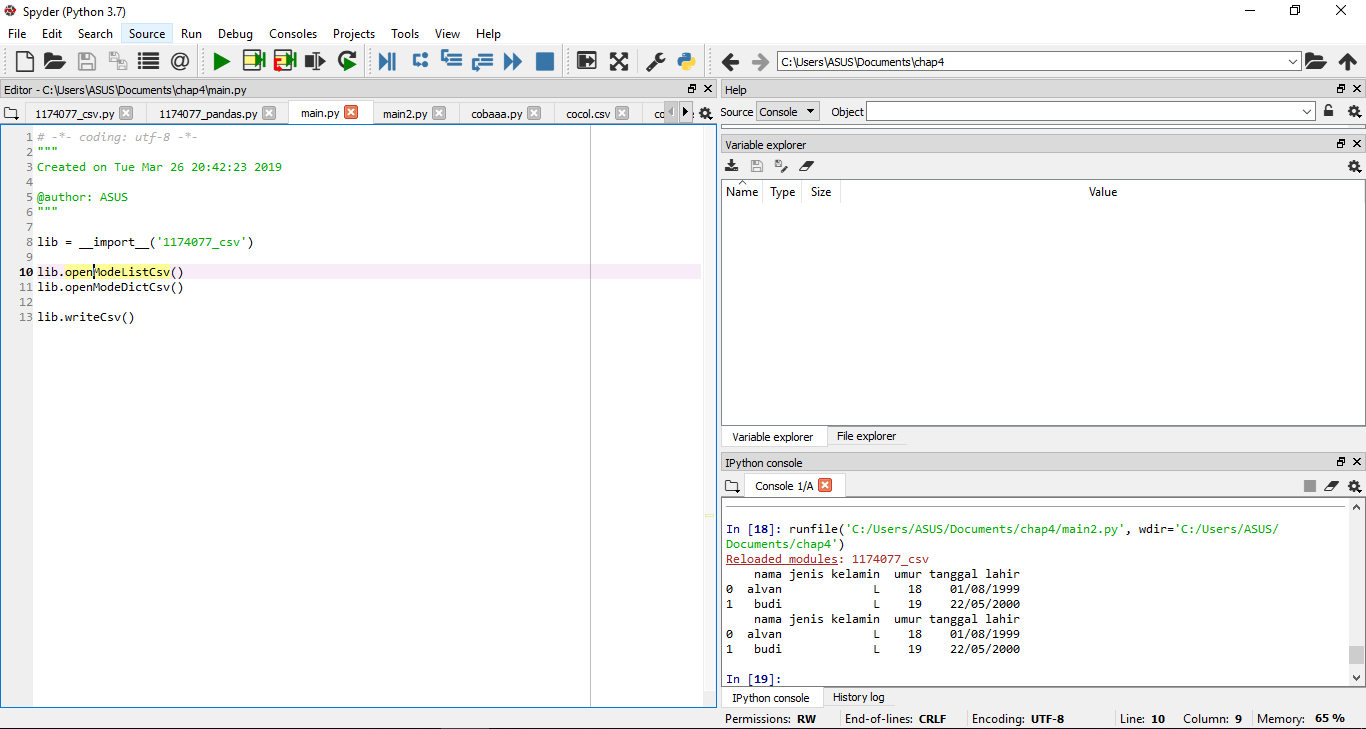
\includegraphics[width=10cm]{figures/4/1174077/Praktek/mainpy.png}
	\centering
\end{figure}
\begin{figure}[!htbp]
	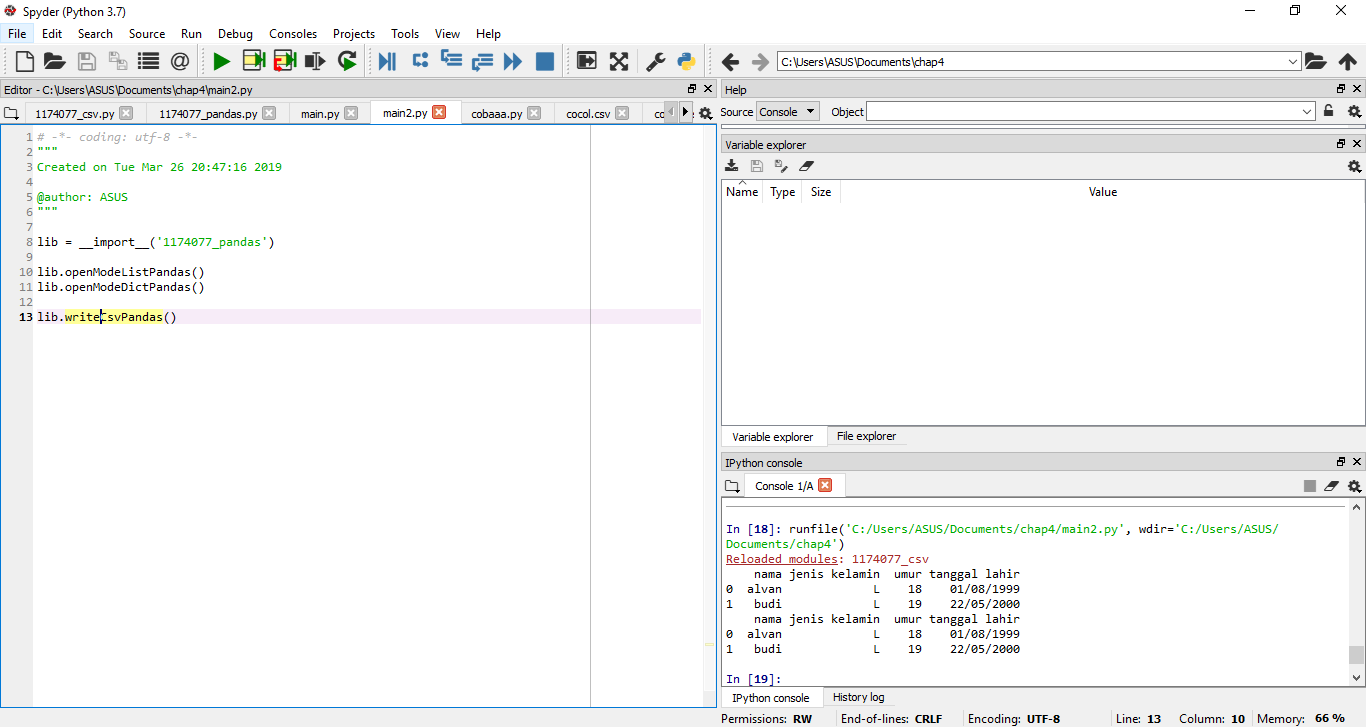
\includegraphics[width=10cm]{figures/4/1174077/Praktek/main2py.png}
	\centering
\end{figure}
\begin{figure}[!htbp]
	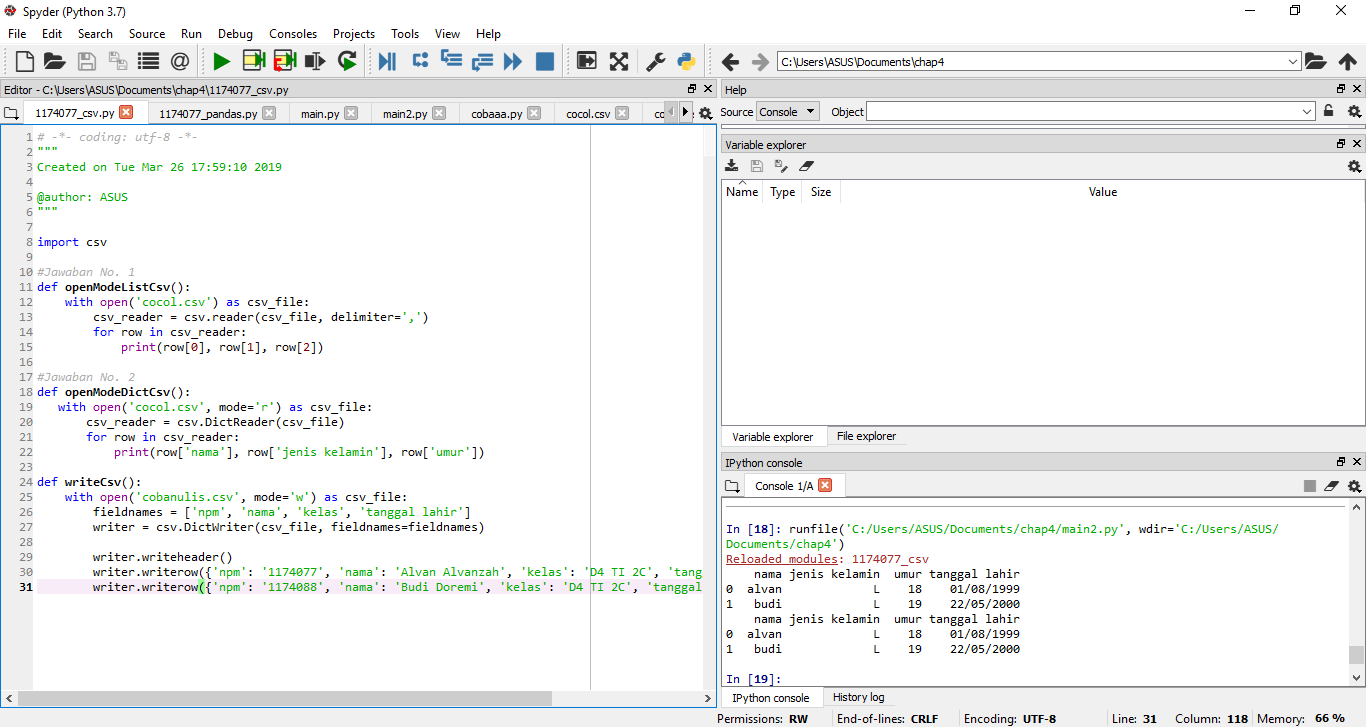
\includegraphics[width=10cm]{figures/4/1174077/Praktek/csv.png}
	\centering
\end{figure}
\begin{figure}[!htbp]
	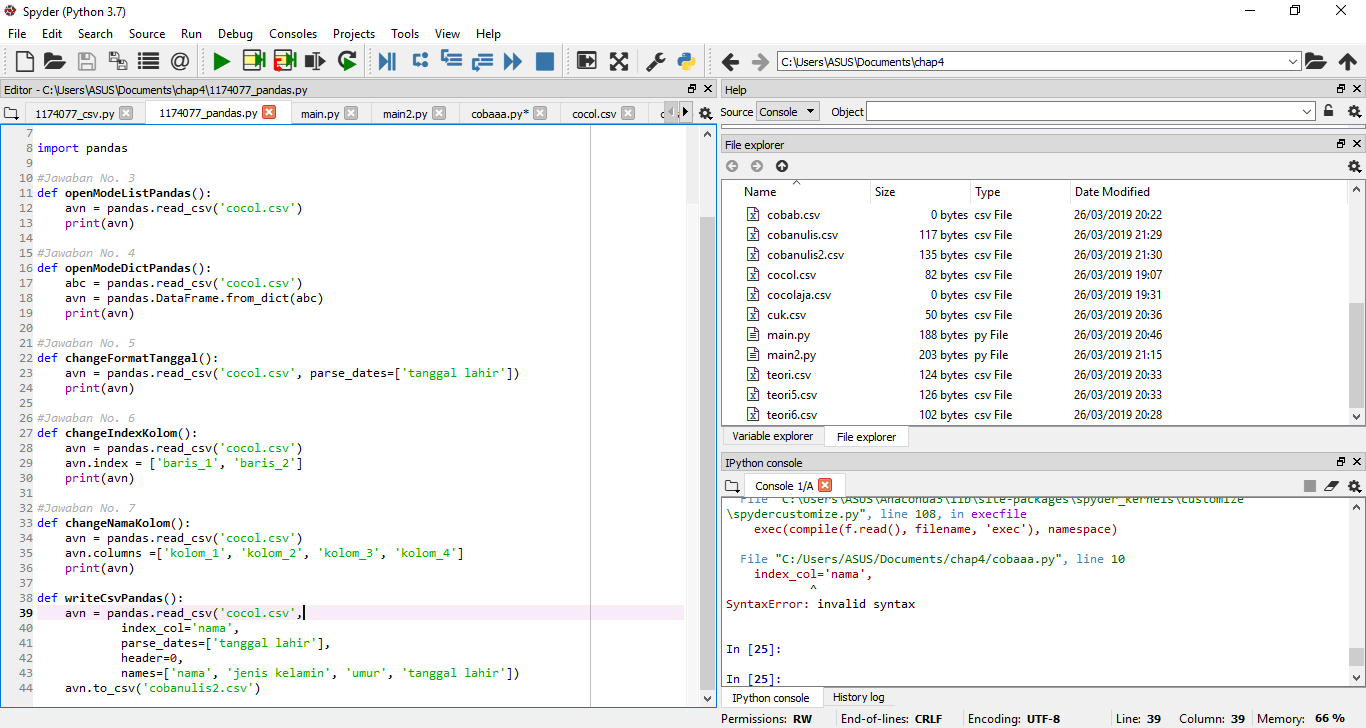
\includegraphics[width=10cm]{figures/4/1174077/Praktek/pandas.png}
	\centering
\end{figure}
%%%%%%%%%%%%%%%%%%%%%%%%%%%%%%%%%%%%%%%%%%%%%%%%%%%%%%%%%%%%%%%%%%%%%%%%%%%%%%%%%%%%%%%%%%%%%%%%%%%%


\title{CHAPTER 4 PRAKTEK}
\author{Handi Hermawan }
\subsection{Keterampilan Pemrograman}
\begin{enumerate}
    \item Buatlah  fungsi  (file  terpisah/library  dengan  nama  \verb|NPM_csv.py|)  untuk  membuka file csv dengan lib csv mode list.
    
   	

    \item Buatlah  fungsi  (file  terpisah/library  dengan  nama  \verb|NPM_csv.py|)  untuk  membuka file csv dengan lib csv mode dictionary.
   	
   	\lstinputlisting[firstline=16, lastline=20]{src/4/1174080/Praktek/1174080_csv.py}

	\item Buatlah fungsi (file terpisah/library dengan nama \verb|NPM_pandas.py|) untuk membuka file csv dengan lib pandas mode list.
	
	\lstinputlisting[firstline=7, lastline=11]{src/4/1174080/Praktek/1174080_pandas.py}
		
	\item Buatlah fungsi (file terpisah/library dengan nama \verb|NPM_pandas.py| untuk membuka file csv dengan lib pandas mode dictionary.

	\lstinputlisting[firstline=13, lastline=16]{src/4/1174080/Praktek/1174080_pandas.py}

	\item Buat fungsi baru di \verb|NPM_pandas.py| untuk mengubah format tanggal menjadi standar dataframe.

	\lstinputlisting[firstline=25, lastline=27]{src/4/1174080/Praktek/1174080_pandas.py}

	\item Buat fungsi baru di \verb|NPM_pandas.py| untuk mengubah index kolom.
	
	\lstinputlisting[firstline=29, lastline=32]{src/4/1174080/Praktek/1174080_pandas.py}
	
	\item Buat fungsi baru di \verb|NPM_pandas.py| untuk mengubah atribut atau nama kolom.
	
	\lstinputlisting[firstline=34, lastline=37]{src/4/1174080/Praktek/1174080_pandas.py}
	
	\item Buat program main.py yang menggunakan library \verb|NPM_csv.py| yang membuat dan membaca file csv.
	
	
	
	\item Buat program main2.py yang menggunakan library \verb|NPM_pandas.py| yang membuat dan membaca file csv.


\end{enumerate} 

\subsection{Keterampilan Penanganan Error}

\begin{enumerate}
	\item Tuliskan peringatan error yang didapat dari mengerjakan praktek ketiga ini,
dan jelaskan cara penanganan error tersebut. dan Buatlah satu fungsi yang
menggunakan gunakan try except untuk menanggulangi error tersebut.
	
	\par NameError adalah exception yang terjadi saat kode melakukan eksekusi terhadap local name atau global name yang tidak terdefinisi. Misalnya saat menjumlahkan variable yang tidak didefinisikan.
	
\end{enumerate}

%%%%%%%%%%%%%%%%%%%%%%%%%%%%%%%%%%%%%%%%%%%%%%%%%%%%%%%%%%%%%%%%%%%%%%%%%%%%%%%%%%%%%%%%%%%%%%%%%%%%%%%%%%%%%


\section{Muhammad Abdul Gani Wijaya}
\subsection{No 1}
Buatlah  fungsi  (file  terpisah/library  dengan  nama  NPMcsv.py)  untuk  membuka file csv dengan lib csv mode list.

\lstinputlisting[caption = Fungsi membuka file CSV dengan lib CSV mode list., firstline=8, lastline=19]{src/4/1174071/Praktek/1174071_csv.py}

\subsection{No 2}
Buatlah  fungsi  (file  terpisah/library  dengan  nama  NPMcsv.py)  untuk  membuka file csv dengan lib csv mode dictionary.

\lstinputlisting[caption =  Fungsi membuka file CSV dengan lib CSV mode dictionary., firstline=21, lastline=30]{src/4/1174071/Praktek/1174071_csv.py}

\subsection{No 3}
Buatlah fungsi (file terpisah/library dengan nama NPMpandas.py) untuk membuka file csv dengan lib pandas mode list.

\lstinputlisting[caption =  Fungsi membuka file CSV dengan lib Pandas mode list., firstline=9, lastline=14]{src/4/1174071/Praktek/1174071_pandas.py}

\subsection{No 4}
Buatlah fungsi (file terpisah/library dengan nama NPMpandas.py) untuk membuka file csv dengan lib pandas mode dictionary.

\lstinputlisting[caption =  Fungsi membuka file CSV dengan lib Pandas mode dictionary., firstline=16, lastline=22]{src/4/1174071/Praktek/1174071_pandas.py}

\subsection{No 5}
Buat fungsi baru di NPMpandas.py untuk mengubah format tanggal menjadi standar dataframe.

\lstinputlisting[caption =  Fungsi mengubah format tanggal menjadi standar dataframe., firstline=24, lastline=29]{src/4/1174071/Praktek/1174071_pandas.py}

\subsection{Soal 6}
Buat fungsi baru di NPMpandas.py untuk mengubah index kolom.

\lstinputlisting[caption =  Fungsi mengubah index kolom., firstline=31, lastline=37]{src/4/1174071/Praktek/1174071_pandas.py}

\subsection{Soal 7}
Buat fungsi baru di NPMpandas.py untuk mengubah atribut atau nama kolom.

\lstinputlisting[caption =  Fungsi untuk mengubah atribut atau nama kolom., firstline=26, lastline=30]{src/4/1174071/Praktek/1174071_pandas.py}

\subsection{Soal 8}
Buat program main.py yang menggunakan library NPMcsv.py yang membuat dan membaca file csv.

\lstinputlisting[caption =  Membuat dan membaca file CSV menggunakan library 1174071pandas., firstline=8, lastline=13]{src/4/1174071/Praktek/main.py}

\subsection{Soal 9}
Buat program main2.py yang menggunakan library NPMpandas.py yang membuat dan membaca file csv.

\lstinputlisting[caption = Membuat dan mmebaca file CSV menggunakan library 1174071pandas., firstline=8, lastline=13]{src/4/1174071/Praktek/main2.py}

\subsection{Kode Program Praktek}
\begin{figure}[ht]
	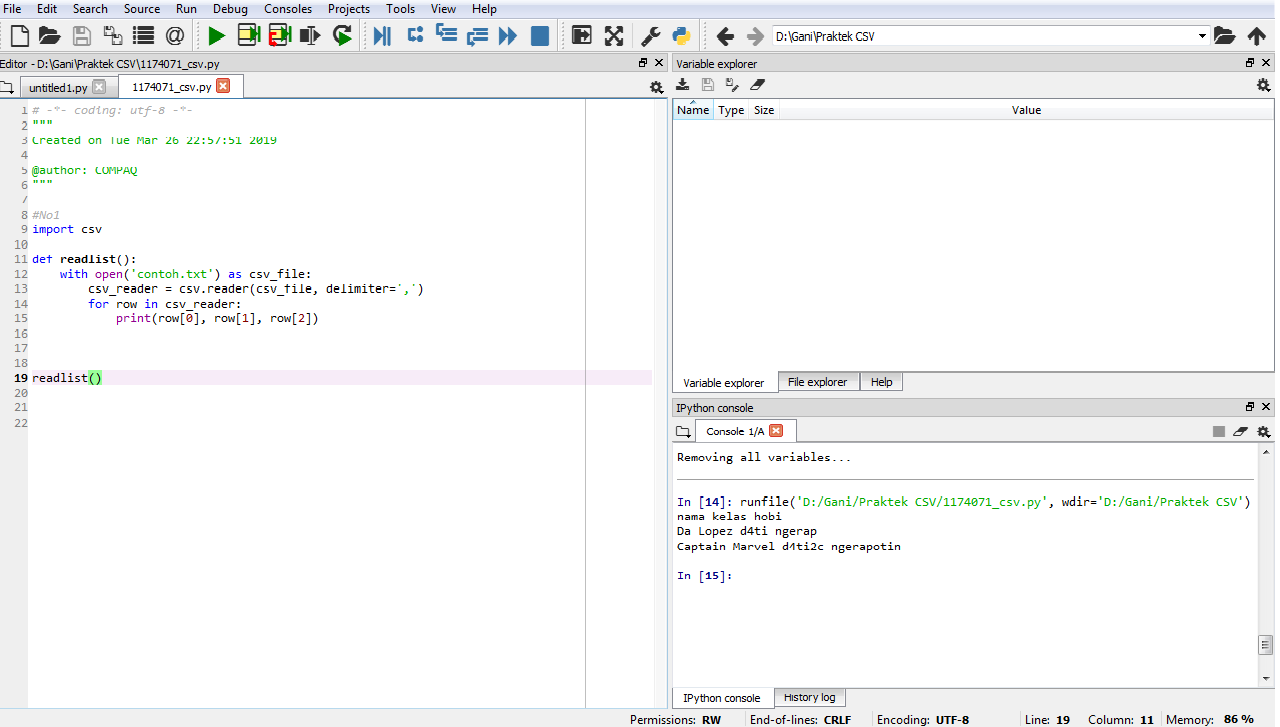
\includegraphics[width=9cm]{figures/4/1174071/Praktek/1174071_csv1.png}
	\centering
\end{figure}
\begin{figure}[ht]
	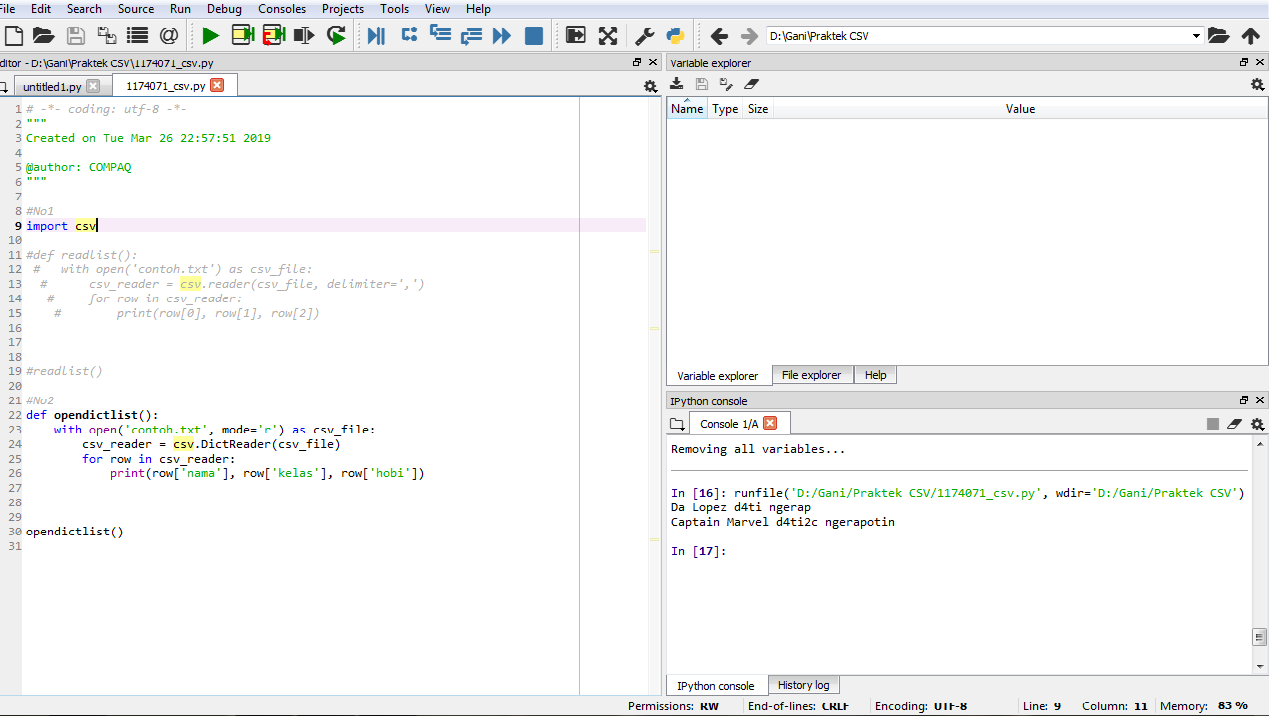
\includegraphics[width=10cm]{figures/4/1174071/Praktek/1174071_csv2.png}
	\centering
\end{figure}
\begin{figure}[ht]
	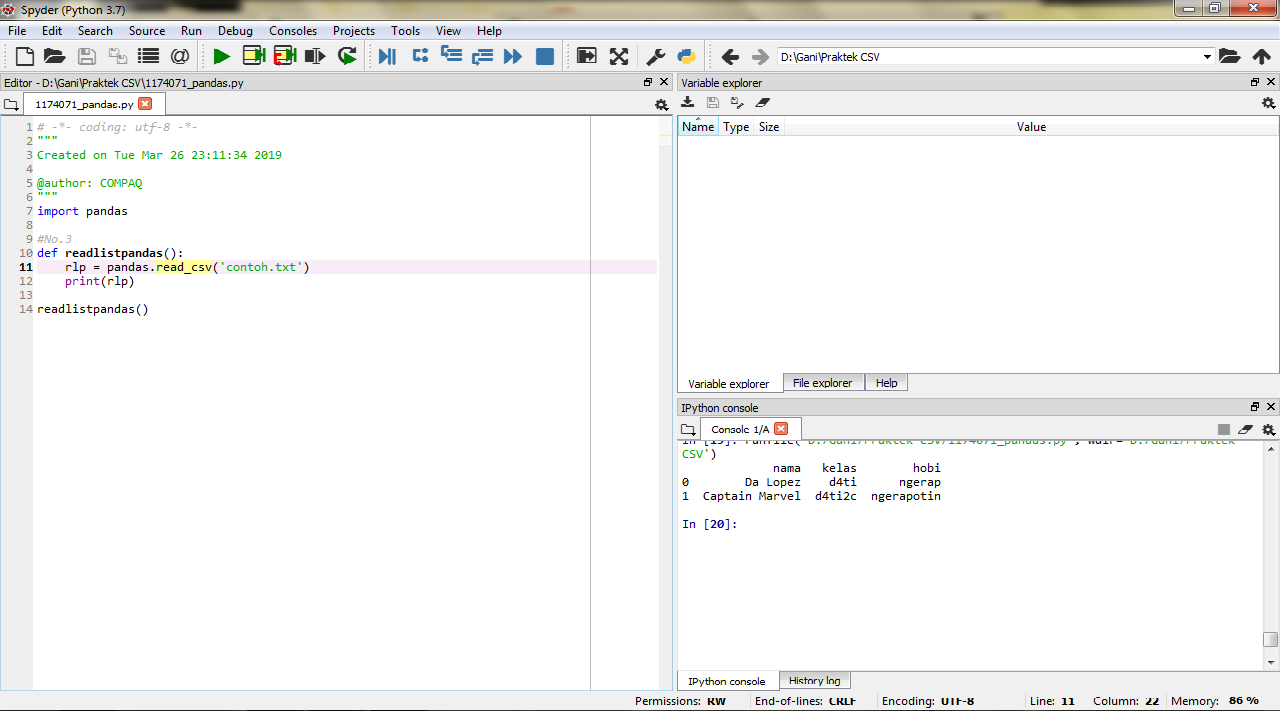
\includegraphics[width=10cm]{figures/4/1174071/Praktek/1174071_pandas3.png}
	\centering
\end{figure}
\begin{figure}[ht]
	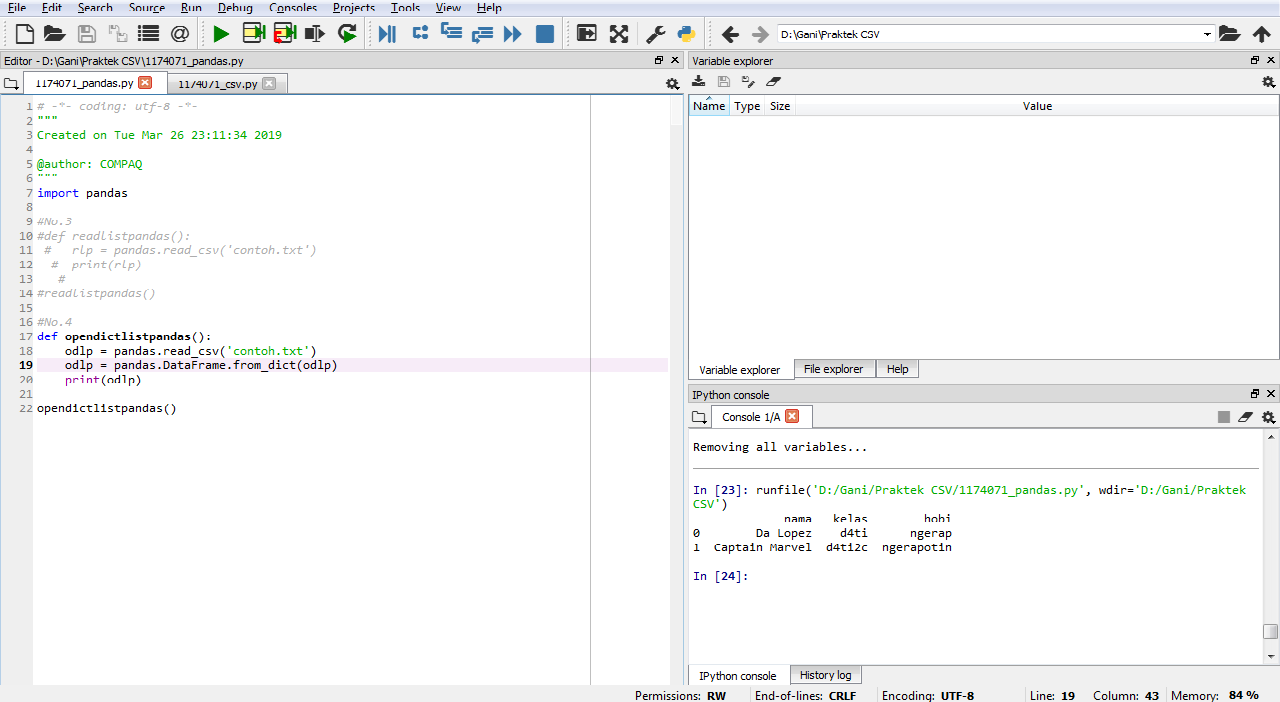
\includegraphics[width=9cm]{figures/4/1174071/Praktek/1174071_pandas4.png}
	\centering
\end{figure}
\begin{figure}[ht]
	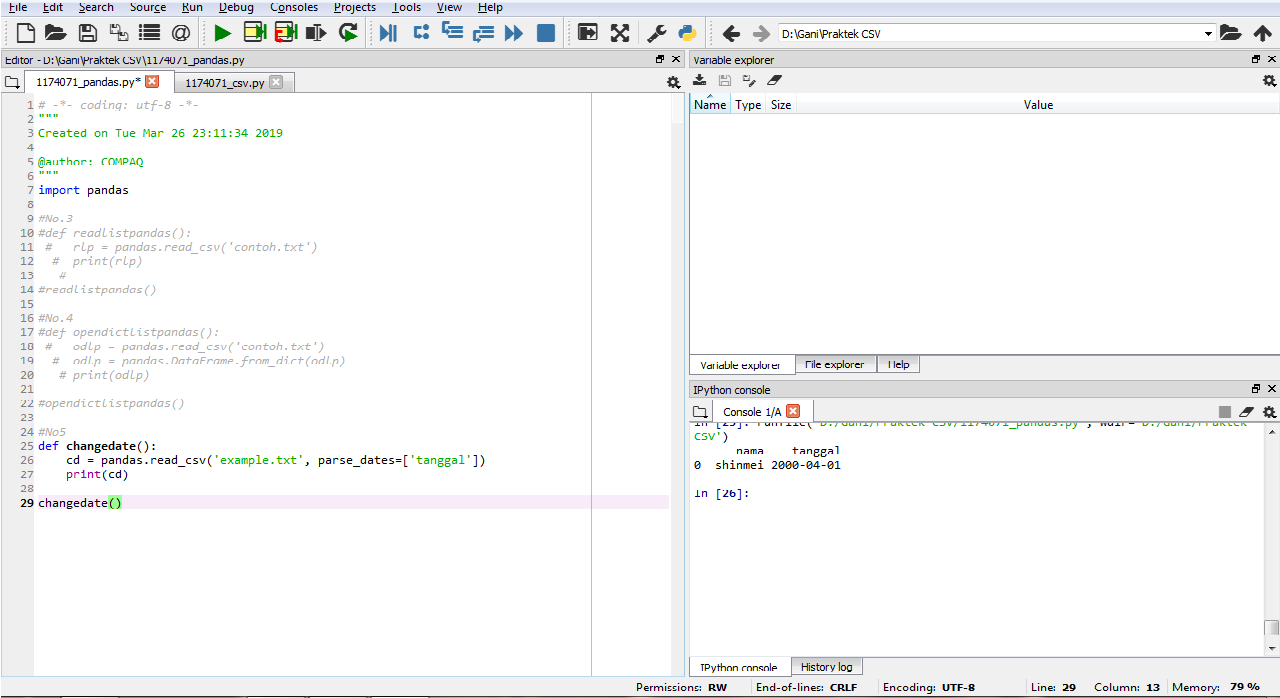
\includegraphics[width=10cm]{figures/4/1174071/Praktek/1174071_pandas5.png}
	\centering
\end{figure}
\begin{figure}[ht]
	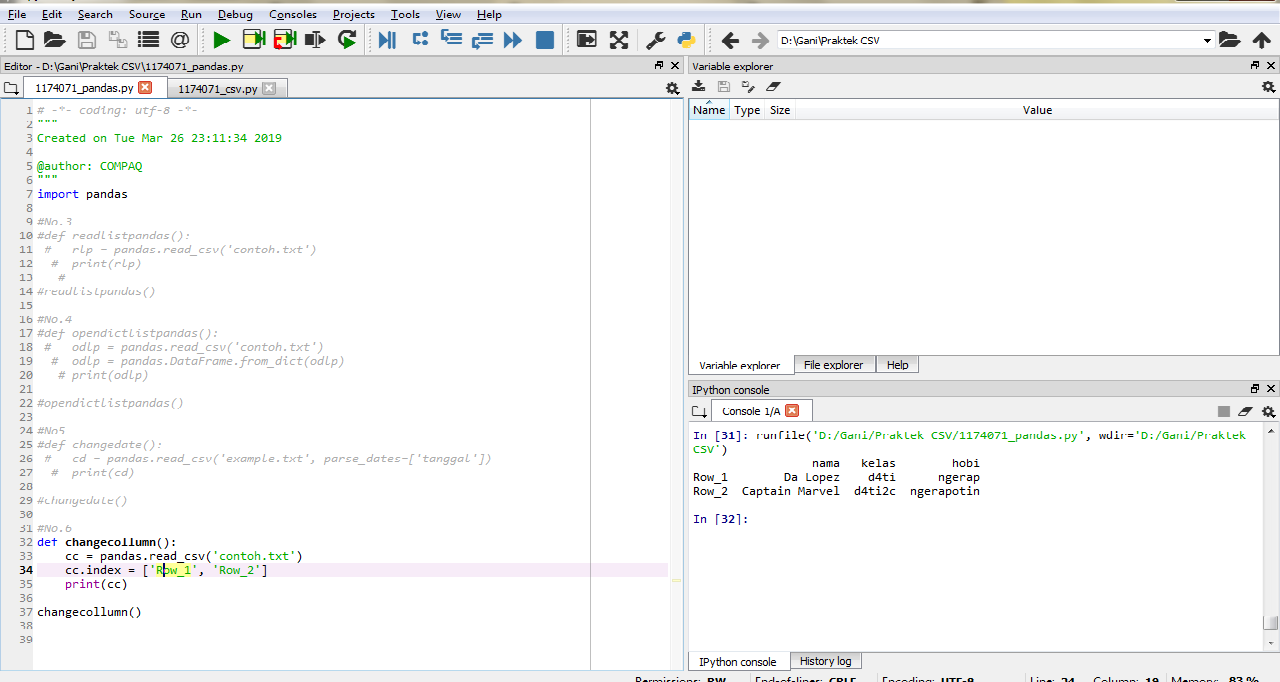
\includegraphics[width=10cm]{figures/4/1174071/Praktek/1174071_pandas6.png}
	\centering
\end{figure}
\begin{figure}[ht]
	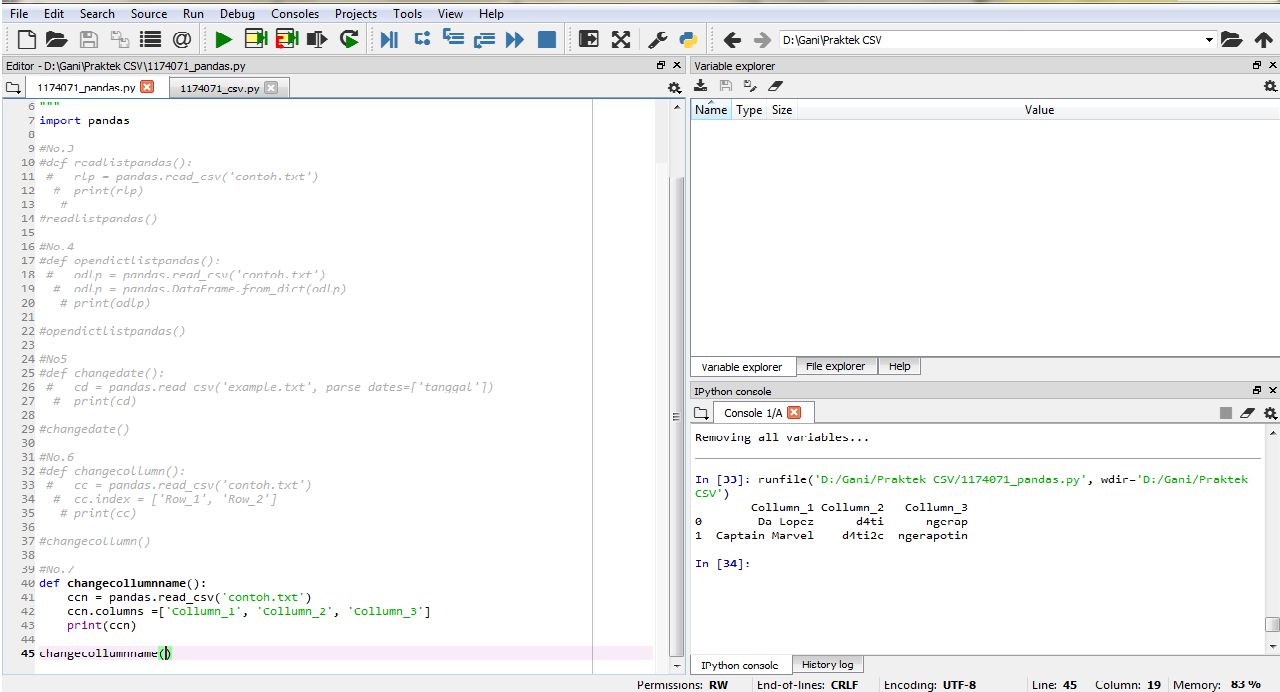
\includegraphics[width=10cm]{figures/4/1174071/Praktek/1174071_pandas7.png}
	\centering
\end{figure}
\begin{figure}[ht]
	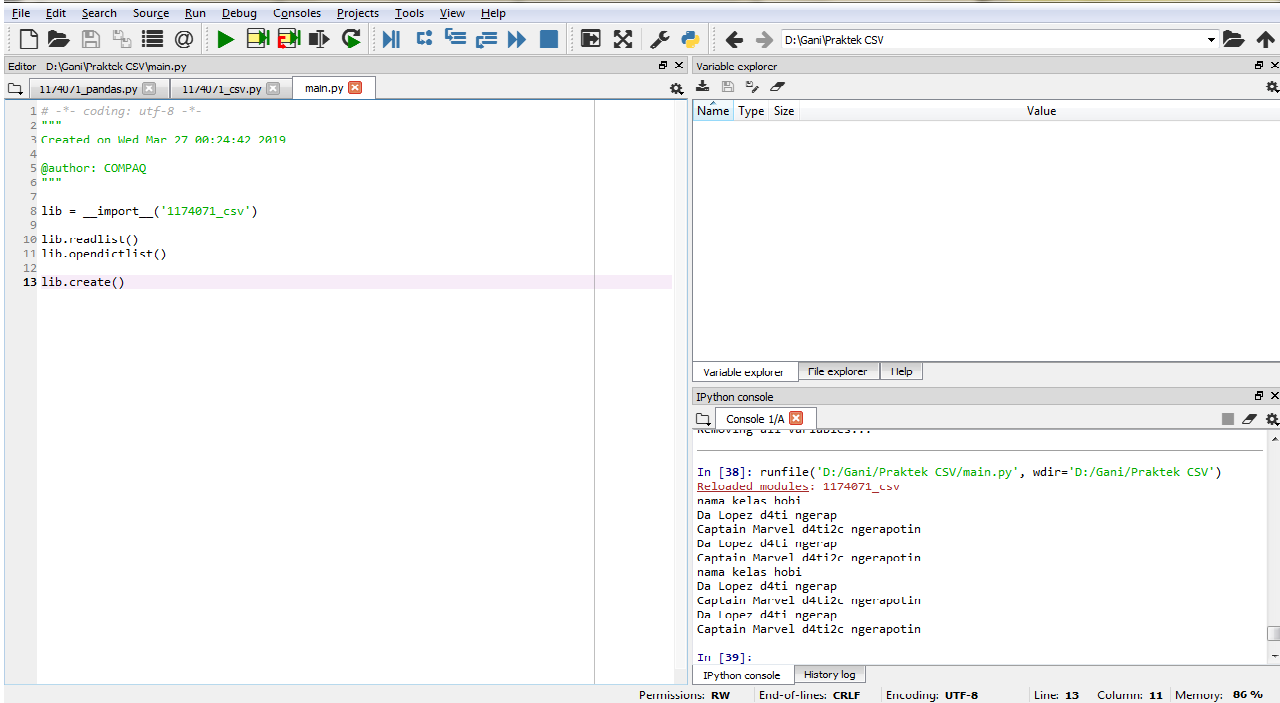
\includegraphics[width=10cm]{figures/4/1174071/Praktek/1174071_main8.png}
	\centering
\end{figure}
\begin{figure}[ht]
	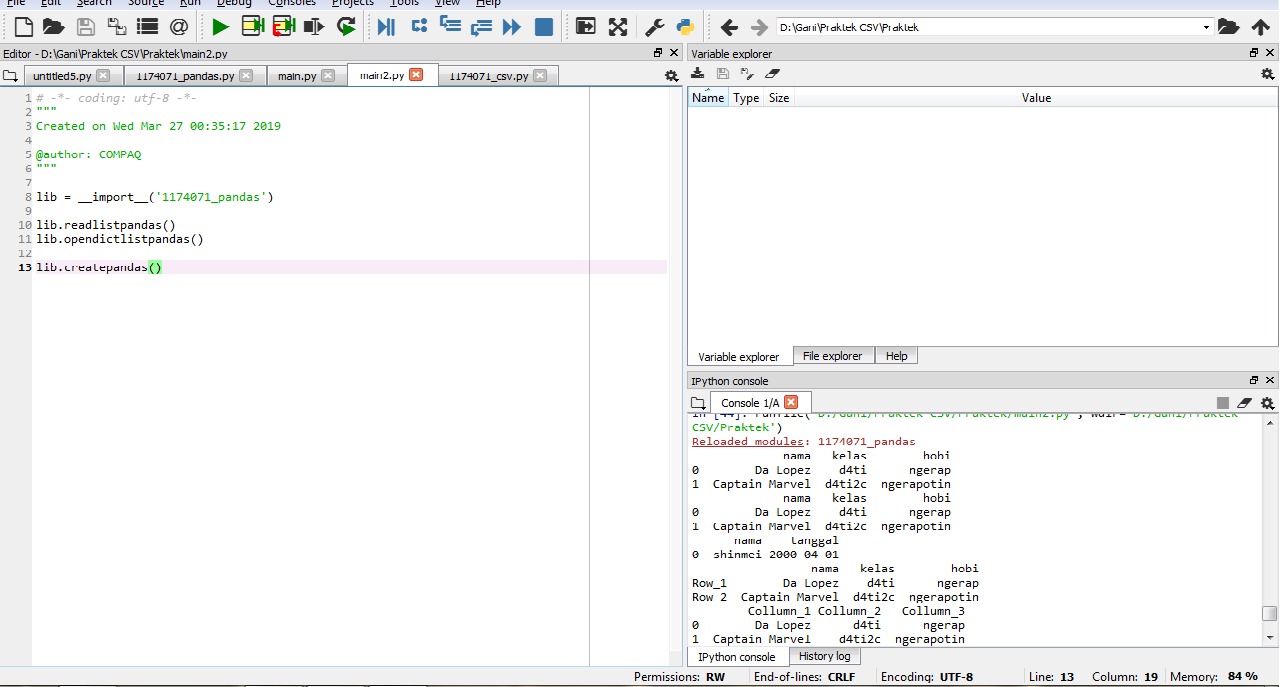
\includegraphics[width=10cm]{figures/4/1174071/Praktek/1174071_main9.png}
	\centering
\end{figure}


%%%%%%%%%%%%%%%%%%%%%%%%%%%%%%%%%%%%%%%%%%%%%%%%%%%%%%%%%%%%%%%%%%%%%%%%%%%%%%%%%%%%%%%%%%%%%%%%%%%%%



\bibliographystyle{IEEEtran}
%\def\bibfont{\normalsize}
\bibliography{references}


%%%%%%%%%%%%%%%
%%  The default LaTeX Index
%%  Don't need to add any commands before \begin{document}
\printindex

%%%% Making an index
%%
%% 1. Make index entries, don't leave any spaces so that they
%% will be sorted correctly.
%%
%% \index{term}
%% \index{term!subterm}
%% \index{term!subterm!subsubterm}
%%
%% 2. Run LaTeX several times to produce <filename>.idx
%%
%% 3. On command line, type  makeindx <filename> which
%% will produce <filename>.ind
%%
%% 4. Type \printindex to make the index appear in your book.
%%
%% 5. If you would like to edit <filename>.ind
%% you may do so. See docs.pdf for more information.
%%
%%%%%%%%%%%%%%%%%%%%%%%%%%%%%%

%%%%%%%%%%%%%% Making Multiple Indices %%%%%%%%%%%%%%%%
%% 1.
%% \usepackage{multind}
%% \makeindex{book}
%% \makeindex{authors}
%% \begin{document}
%%
%% 2.
%% % add index terms to your book, ie,
%% \index{book}{A term to go to the topic index}
%% \index{authors}{Put this author in the author index}
%%
%% \index{book}{Cows}
%% \index{book}{Cows!Jersey}
%% \index{book}{Cows!Jersey!Brown}
%%
%% \index{author}{Douglas Adams}
%% \index{author}{Boethius}
%% \index{author}{Mark Twain}
%%
%% 3. On command line type
%% makeindex topic
%% makeindex authors
%%
%% 4.
%% this is a Wiley command to make the indices print:
%% \multiprintindex{book}{Topic index}
%% \multiprintindex{authors}{Author index}

\end{document}

